\section{Conjunto de entrenamiento}
\subsection{Descripción}
Uno de los principales retos al trabajar con redes neuronales es la obtención de grandes conjuntos de entrenamiento que permitan mejores resultados, para el problema de reconocimiento de expresiones matemáticas existe una competencia llamada \textbf{Competition on Recognition of Online Handwritten Mathematical Expressions (CROHME)} que pone disponible de manera libre un conjunto de entrenamiento con mas de diez mil expresiones matemáticas escritas a mano provenientes de muchos usuarios voluntarios de distintos países mezclando los conjuntos de entrenamiento de 3 competencias CROHME. Se le pidió a los voluntarios copiar expresiones impresas de un \texttt{corpus} de expresiones. El corpus ha sido diseñado para cubrir la diversidad compuesta por las distintas tareas elegidas de un corpora matemático y de expresiones embebidas en páginas de wikipedia. Distintos dispositivos han sido utilizados (plumas digitales de distintas tecnologías, dispositivos de entrada como pizarrones blancos, tablets con pantalla sensible) de tal modo que distintas escalas y resoluciones son usadas %\cite{}.

\begin{figure}[h]
	\centering
	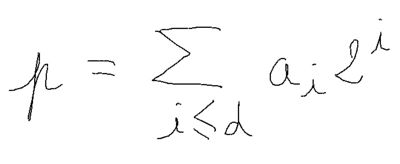
\includegraphics[width=0.4\textwidth]{capitulo5/dataset/crohme.jpg}
	\caption{Imagen de ejemplo del conjunto de datos de CROHME}
	\label{fig:crohme}
\end{figure}
\newpage
A pesar de parecer un conjunto de datos prometedor para el desarrollo del presente trabajo terminal se deben considerar factores como el ruido que puede tener una imagen a partir de una fotografía tomada con un smartphone, por lo que se considera también otro conjunto de entrenamiento llamado \textbf{im2latex-100k} \cite{imagetolatex}. El cual a diferencia de CROHME no se enfoca en expresiones matemáticas escritas a mano sino extraídas de documentos generados por computadora como pueden ser libros o artículos impresos. \cite{kanervisto_anssi_2016_56198}.

\begin{figure}[h]
	\centering
	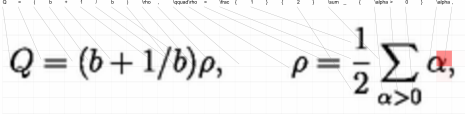
\includegraphics[width=0.4\textwidth]{capitulo5/dataset/Dengetal.png}
	\caption{Imagen de ejemplo del conjunto de datos de Im2latex-100k}
	\label{fig:deng}
\end{figure}

Para la segunda parte de este trabajo terminal se utilizarán algunas métricas de evaluación donde el principal parámetro será la precisión. Se propondrán varias arquitecturas de redes neuronales de prueba y se entrenarán con ambos conjuntos para así comparar la precisión que ofrecería un modelo entrenado por cada conjunto, una vez hecho esto se elijirá el modelo y el conjunto que presente mayor precisión.  